\documentclass[]{article}
\usepackage{lmodern}
\usepackage{amssymb,amsmath}
\usepackage{ifxetex,ifluatex}
\usepackage{fixltx2e} % provides \textsubscript
\ifnum 0\ifxetex 1\fi\ifluatex 1\fi=0 % if pdftex
  \usepackage[T1]{fontenc}
  \usepackage[utf8]{inputenc}
\else % if luatex or xelatex
  \ifxetex
    \usepackage{mathspec}
  \else
    \usepackage{fontspec}
  \fi
  \defaultfontfeatures{Ligatures=TeX,Scale=MatchLowercase}
\fi
% use upquote if available, for straight quotes in verbatim environments
\IfFileExists{upquote.sty}{\usepackage{upquote}}{}
% use microtype if available
\IfFileExists{microtype.sty}{%
\usepackage{microtype}
\UseMicrotypeSet[protrusion]{basicmath} % disable protrusion for tt fonts
}{}
\usepackage[margin=2.54cm]{geometry}
\usepackage{hyperref}
\hypersetup{unicode=true,
            pdftitle={Assignment 5: Data Visualization},
            pdfauthor={Sarah Ko},
            pdfborder={0 0 0},
            breaklinks=true}
\urlstyle{same}  % don't use monospace font for urls
\usepackage{color}
\usepackage{fancyvrb}
\newcommand{\VerbBar}{|}
\newcommand{\VERB}{\Verb[commandchars=\\\{\}]}
\DefineVerbatimEnvironment{Highlighting}{Verbatim}{commandchars=\\\{\}}
% Add ',fontsize=\small' for more characters per line
\usepackage{framed}
\definecolor{shadecolor}{RGB}{248,248,248}
\newenvironment{Shaded}{\begin{snugshade}}{\end{snugshade}}
\newcommand{\KeywordTok}[1]{\textcolor[rgb]{0.13,0.29,0.53}{\textbf{#1}}}
\newcommand{\DataTypeTok}[1]{\textcolor[rgb]{0.13,0.29,0.53}{#1}}
\newcommand{\DecValTok}[1]{\textcolor[rgb]{0.00,0.00,0.81}{#1}}
\newcommand{\BaseNTok}[1]{\textcolor[rgb]{0.00,0.00,0.81}{#1}}
\newcommand{\FloatTok}[1]{\textcolor[rgb]{0.00,0.00,0.81}{#1}}
\newcommand{\ConstantTok}[1]{\textcolor[rgb]{0.00,0.00,0.00}{#1}}
\newcommand{\CharTok}[1]{\textcolor[rgb]{0.31,0.60,0.02}{#1}}
\newcommand{\SpecialCharTok}[1]{\textcolor[rgb]{0.00,0.00,0.00}{#1}}
\newcommand{\StringTok}[1]{\textcolor[rgb]{0.31,0.60,0.02}{#1}}
\newcommand{\VerbatimStringTok}[1]{\textcolor[rgb]{0.31,0.60,0.02}{#1}}
\newcommand{\SpecialStringTok}[1]{\textcolor[rgb]{0.31,0.60,0.02}{#1}}
\newcommand{\ImportTok}[1]{#1}
\newcommand{\CommentTok}[1]{\textcolor[rgb]{0.56,0.35,0.01}{\textit{#1}}}
\newcommand{\DocumentationTok}[1]{\textcolor[rgb]{0.56,0.35,0.01}{\textbf{\textit{#1}}}}
\newcommand{\AnnotationTok}[1]{\textcolor[rgb]{0.56,0.35,0.01}{\textbf{\textit{#1}}}}
\newcommand{\CommentVarTok}[1]{\textcolor[rgb]{0.56,0.35,0.01}{\textbf{\textit{#1}}}}
\newcommand{\OtherTok}[1]{\textcolor[rgb]{0.56,0.35,0.01}{#1}}
\newcommand{\FunctionTok}[1]{\textcolor[rgb]{0.00,0.00,0.00}{#1}}
\newcommand{\VariableTok}[1]{\textcolor[rgb]{0.00,0.00,0.00}{#1}}
\newcommand{\ControlFlowTok}[1]{\textcolor[rgb]{0.13,0.29,0.53}{\textbf{#1}}}
\newcommand{\OperatorTok}[1]{\textcolor[rgb]{0.81,0.36,0.00}{\textbf{#1}}}
\newcommand{\BuiltInTok}[1]{#1}
\newcommand{\ExtensionTok}[1]{#1}
\newcommand{\PreprocessorTok}[1]{\textcolor[rgb]{0.56,0.35,0.01}{\textit{#1}}}
\newcommand{\AttributeTok}[1]{\textcolor[rgb]{0.77,0.63,0.00}{#1}}
\newcommand{\RegionMarkerTok}[1]{#1}
\newcommand{\InformationTok}[1]{\textcolor[rgb]{0.56,0.35,0.01}{\textbf{\textit{#1}}}}
\newcommand{\WarningTok}[1]{\textcolor[rgb]{0.56,0.35,0.01}{\textbf{\textit{#1}}}}
\newcommand{\AlertTok}[1]{\textcolor[rgb]{0.94,0.16,0.16}{#1}}
\newcommand{\ErrorTok}[1]{\textcolor[rgb]{0.64,0.00,0.00}{\textbf{#1}}}
\newcommand{\NormalTok}[1]{#1}
\usepackage{graphicx,grffile}
\makeatletter
\def\maxwidth{\ifdim\Gin@nat@width>\linewidth\linewidth\else\Gin@nat@width\fi}
\def\maxheight{\ifdim\Gin@nat@height>\textheight\textheight\else\Gin@nat@height\fi}
\makeatother
% Scale images if necessary, so that they will not overflow the page
% margins by default, and it is still possible to overwrite the defaults
% using explicit options in \includegraphics[width, height, ...]{}
\setkeys{Gin}{width=\maxwidth,height=\maxheight,keepaspectratio}
\IfFileExists{parskip.sty}{%
\usepackage{parskip}
}{% else
\setlength{\parindent}{0pt}
\setlength{\parskip}{6pt plus 2pt minus 1pt}
}
\setlength{\emergencystretch}{3em}  % prevent overfull lines
\providecommand{\tightlist}{%
  \setlength{\itemsep}{0pt}\setlength{\parskip}{0pt}}
\setcounter{secnumdepth}{0}
% Redefines (sub)paragraphs to behave more like sections
\ifx\paragraph\undefined\else
\let\oldparagraph\paragraph
\renewcommand{\paragraph}[1]{\oldparagraph{#1}\mbox{}}
\fi
\ifx\subparagraph\undefined\else
\let\oldsubparagraph\subparagraph
\renewcommand{\subparagraph}[1]{\oldsubparagraph{#1}\mbox{}}
\fi

%%% Use protect on footnotes to avoid problems with footnotes in titles
\let\rmarkdownfootnote\footnote%
\def\footnote{\protect\rmarkdownfootnote}

%%% Change title format to be more compact
\usepackage{titling}

% Create subtitle command for use in maketitle
\newcommand{\subtitle}[1]{
  \posttitle{
    \begin{center}\large#1\end{center}
    }
}

\setlength{\droptitle}{-2em}

  \title{Assignment 5: Data Visualization}
    \pretitle{\vspace{\droptitle}\centering\huge}
  \posttitle{\par}
    \author{Sarah Ko}
    \preauthor{\centering\large\emph}
  \postauthor{\par}
    \date{}
    \predate{}\postdate{}
  

\begin{document}
\maketitle

\subsection{OVERVIEW}\label{overview}

This exercise accompanies the lessons in Environmental Data Analytics
(ENV872L) on data wrangling.

\subsection{Directions}\label{directions}

\begin{enumerate}
\def\labelenumi{\arabic{enumi}.}
\tightlist
\item
  Change ``Student Name'' on line 3 (above) with your name.
\item
  Use the lesson as a guide. It contains code that can be modified to
  complete the assignment.
\item
  Work through the steps, \textbf{creating code and output} that fulfill
  each instruction.
\item
  Be sure to \textbf{answer the questions} in this assignment document.
  Space for your answers is provided in this document and is indicated
  by the ``\textgreater{}'' character. If you need a second paragraph be
  sure to start the first line with ``\textgreater{}''. You should
  notice that the answer is highlighted in green by RStudio.
\item
  When you have completed the assignment, \textbf{Knit} the text and
  code into a single PDF file. You will need to have the correct
  software installed to do this (see Software Installation Guide) Press
  the \texttt{Knit} button in the RStudio scripting panel. This will
  save the PDF output in your Assignments folder.
\item
  After Knitting, please submit the completed exercise (PDF file) to the
  dropbox in Sakai. Please add your last name into the file name (e.g.,
  ``Salk\_A04\_DataWrangling.pdf'') prior to submission.
\end{enumerate}

The completed exercise is due on Tuesday, 19 February, 2019 before class
begins.

\subsection{Set up your session}\label{set-up-your-session}

\begin{enumerate}
\def\labelenumi{\arabic{enumi}.}
\item
  Set up your session. Upload the NTL-LTER processed data files for
  chemistry/physics for Peter and Paul Lakes (tidy and gathered), the
  USGS stream gauge dataset, and the EPA Ecotox dataset for
  Neonicotinoids.
\item
  Make sure R is reading dates as date format, not something else (hint:
  remember that dates were an issue for the USGS gauge data).
\end{enumerate}

\begin{Shaded}
\begin{Highlighting}[]
\CommentTok{#load packages}
\KeywordTok{library}\NormalTok{(tidyverse)}
\end{Highlighting}
\end{Shaded}

\begin{verbatim}
## Warning: package 'tidyverse' was built under R version 3.5.2
\end{verbatim}

\begin{verbatim}
## -- Attaching packages -------------------------------------------------------------- tidyverse 1.2.1 --
\end{verbatim}

\begin{verbatim}
## v ggplot2 3.1.0     v purrr   0.3.0
## v tibble  2.0.1     v dplyr   0.7.8
## v tidyr   0.8.2     v stringr 1.3.1
## v readr   1.3.1     v forcats 0.3.0
\end{verbatim}

\begin{verbatim}
## Warning: package 'ggplot2' was built under R version 3.5.2
\end{verbatim}

\begin{verbatim}
## Warning: package 'tibble' was built under R version 3.5.2
\end{verbatim}

\begin{verbatim}
## Warning: package 'tidyr' was built under R version 3.5.2
\end{verbatim}

\begin{verbatim}
## Warning: package 'readr' was built under R version 3.5.2
\end{verbatim}

\begin{verbatim}
## Warning: package 'purrr' was built under R version 3.5.2
\end{verbatim}

\begin{verbatim}
## Warning: package 'dplyr' was built under R version 3.5.2
\end{verbatim}

\begin{verbatim}
## -- Conflicts ----------------------------------------------------------------- tidyverse_conflicts() --
## x dplyr::filter() masks stats::filter()
## x dplyr::lag()    masks stats::lag()
\end{verbatim}

\begin{Shaded}
\begin{Highlighting}[]
\KeywordTok{library}\NormalTok{(viridis)}
\end{Highlighting}
\end{Shaded}

\begin{verbatim}
## Warning: package 'viridis' was built under R version 3.5.2
\end{verbatim}

\begin{verbatim}
## Loading required package: viridisLite
\end{verbatim}

\begin{Shaded}
\begin{Highlighting}[]
\KeywordTok{library}\NormalTok{(RColorBrewer)}
\end{Highlighting}
\end{Shaded}

\begin{verbatim}
## Warning: package 'RColorBrewer' was built under R version 3.5.2
\end{verbatim}

\begin{Shaded}
\begin{Highlighting}[]
\KeywordTok{library}\NormalTok{(colormap)}
\end{Highlighting}
\end{Shaded}

\begin{verbatim}
## Warning: package 'colormap' was built under R version 3.5.2
\end{verbatim}

\begin{Shaded}
\begin{Highlighting}[]
\KeywordTok{library}\NormalTok{(tidyr)}
\KeywordTok{library}\NormalTok{(ggpubr)}
\end{Highlighting}
\end{Shaded}

\begin{verbatim}
## Warning: package 'ggpubr' was built under R version 3.5.2
\end{verbatim}

\begin{verbatim}
## Loading required package: magrittr
\end{verbatim}

\begin{verbatim}
## 
## Attaching package: 'magrittr'
\end{verbatim}

\begin{verbatim}
## The following object is masked from 'package:purrr':
## 
##     set_names
\end{verbatim}

\begin{verbatim}
## The following object is masked from 'package:tidyr':
## 
##     extract
\end{verbatim}

\begin{Shaded}
\begin{Highlighting}[]
\CommentTok{#1}

\CommentTok{# get working directory}
\KeywordTok{getwd}\NormalTok{()}
\end{Highlighting}
\end{Shaded}

\begin{verbatim}
## [1] "C:/Users/Sarah/Documents/Duke/Year 2/Spring 2019/Data Analytics/Environmental_Data_Analytics"
\end{verbatim}

\begin{Shaded}
\begin{Highlighting}[]
\CommentTok{# set wd to the filepath of Environmental_Data_Analytics to use relative filepath}

\NormalTok{PeterPaul.Gathered <-}\StringTok{ }\KeywordTok{read.csv}\NormalTok{(}\StringTok{"./Data/Processed/NTL-LTER_Lake_Nutrients_PeterPaulGathered_Processed.csv"}\NormalTok{)}

\NormalTok{Stream.Raw <-}\StringTok{ }\KeywordTok{read.csv}\NormalTok{(}\StringTok{"./Data/Raw/USGS_Site02085000_Flow_Raw.csv"}\NormalTok{)}

\NormalTok{Neonicotinoids.Raw <-}\StringTok{ }\KeywordTok{read.csv}\NormalTok{(}\StringTok{"./Data/Raw/ECOTOX_Neonicotinoids_Mortality_raw.csv"}\NormalTok{)}

\CommentTok{# check that the dates fall within the reasonable timeframe}

\KeywordTok{head}\NormalTok{(PeterPaul.Gathered}\OperatorTok{$}\NormalTok{sampledate)}
\end{Highlighting}
\end{Shaded}

\begin{verbatim}
## [1] 1991-05-20 1991-05-20 1991-05-20 1991-05-20 1991-05-20 1991-05-20
## 778 Levels: 1991-05-20 1991-05-27 1991-05-28 1991-06-03 ... 2016-08-16
\end{verbatim}

\begin{Shaded}
\begin{Highlighting}[]
\KeywordTok{head}\NormalTok{(Stream.Raw}\OperatorTok{$}\NormalTok{datetime)}
\end{Highlighting}
\end{Shaded}

\begin{verbatim}
## [1] 1/1/28 1/2/28 1/3/28 1/4/28 1/5/28 1/6/28
## 33216 Levels: 1/1/00 1/1/01 1/1/02 1/1/03 1/1/04 1/1/05 1/1/06 ... 9/9/99
\end{verbatim}

\begin{Shaded}
\begin{Highlighting}[]
\KeywordTok{head}\NormalTok{(Neonicotinoids.Raw}\OperatorTok{$}\NormalTok{Pub..Year)}
\end{Highlighting}
\end{Shaded}

\begin{verbatim}
## [1] 2013 2017 2013 2013 2016 2016
\end{verbatim}

\begin{Shaded}
\begin{Highlighting}[]
\CommentTok{# fix the dates in Stream.Raw}

\CommentTok{# change the class to date}
\NormalTok{Stream.Raw}\OperatorTok{$}\NormalTok{datetime <-}\StringTok{ }\KeywordTok{as.Date}\NormalTok{(Stream.Raw}\OperatorTok{$}\NormalTok{datetime, }\DataTypeTok{format =} \StringTok{"%m/%d/%y"}\NormalTok{)}

\CommentTok{# format the dates as 6 character string: year/month/date}
\NormalTok{Stream.Raw}\OperatorTok{$}\NormalTok{datetime <-}\StringTok{ }\KeywordTok{format}\NormalTok{(Stream.Raw}\OperatorTok{$}\NormalTok{datetime, }\StringTok{"%y%m%d"}\NormalTok{)}

\CommentTok{# create a function. }
\CommentTok{# paste0 amends the components together}
\CommentTok{# checks if the date is after Dec 31, 2018 (the last possible day in the dataset). if its over, the date is actually in the 1900s, so start the string as 19, else set the string as 20. }
\NormalTok{create.early.dates <-}\StringTok{ }\NormalTok{(}\ControlFlowTok{function}\NormalTok{(d) \{}
       \KeywordTok{paste0}\NormalTok{(}\KeywordTok{ifelse}\NormalTok{(d }\OperatorTok{>}\StringTok{ }\DecValTok{181231}\NormalTok{,}\StringTok{"19"}\NormalTok{,}\StringTok{"20"}\NormalTok{),d)}
\NormalTok{       \})}

\CommentTok{# create the new dates, reformat}
\NormalTok{Stream.Raw}\OperatorTok{$}\NormalTok{datetime <-}\StringTok{ }\KeywordTok{create.early.dates}\NormalTok{(Stream.Raw}\OperatorTok{$}\NormalTok{datetime)}
\NormalTok{Stream.Raw}\OperatorTok{$}\NormalTok{datetime <-}\StringTok{ }\KeywordTok{as.Date}\NormalTok{(Stream.Raw}\OperatorTok{$}\NormalTok{datetime, }\DataTypeTok{format =} \StringTok{"%Y%m%d"}\NormalTok{) }

\CommentTok{#2}

\CommentTok{# check the class of the date columns}

\KeywordTok{class}\NormalTok{(PeterPaul.Gathered}\OperatorTok{$}\NormalTok{sampledate)}
\end{Highlighting}
\end{Shaded}

\begin{verbatim}
## [1] "factor"
\end{verbatim}

\begin{Shaded}
\begin{Highlighting}[]
\KeywordTok{class}\NormalTok{(Stream.Raw}\OperatorTok{$}\NormalTok{datetime)}
\end{Highlighting}
\end{Shaded}

\begin{verbatim}
## [1] "Date"
\end{verbatim}

\begin{Shaded}
\begin{Highlighting}[]
\KeywordTok{class}\NormalTok{(Neonicotinoids.Raw}\OperatorTok{$}\NormalTok{Pub..Year)}
\end{Highlighting}
\end{Shaded}

\begin{verbatim}
## [1] "integer"
\end{verbatim}

\begin{Shaded}
\begin{Highlighting}[]
\CommentTok{# change class date. must define original format of data}
\NormalTok{PeterPaul.Gathered}\OperatorTok{$}\NormalTok{sampledate <-}\StringTok{ }\KeywordTok{as.Date}\NormalTok{(PeterPaul.Gathered}\OperatorTok{$}\NormalTok{sampledate, }\DataTypeTok{format =} \StringTok{"%Y-%m-%d"}\NormalTok{)}

\CommentTok{# the Neonicotinoid column Pub..Year is already an integer, and does not have a month/day associated with it}

\CommentTok{# confirm class of the date columns}

\KeywordTok{class}\NormalTok{(PeterPaul.Gathered}\OperatorTok{$}\NormalTok{sampledate)}
\end{Highlighting}
\end{Shaded}

\begin{verbatim}
## [1] "Date"
\end{verbatim}

\begin{Shaded}
\begin{Highlighting}[]
\KeywordTok{class}\NormalTok{(Stream.Raw}\OperatorTok{$}\NormalTok{datetime)}
\end{Highlighting}
\end{Shaded}

\begin{verbatim}
## [1] "Date"
\end{verbatim}

\subsection{Define your theme}\label{define-your-theme}

\begin{enumerate}
\def\labelenumi{\arabic{enumi}.}
\setcounter{enumi}{2}
\tightlist
\item
  Build a theme and set it as your default theme.
\end{enumerate}

\begin{Shaded}
\begin{Highlighting}[]
\CommentTok{#3}

\NormalTok{SKotheme <-}\StringTok{ }\KeywordTok{theme_gray}\NormalTok{(}\DataTypeTok{base_size =} \DecValTok{15}\NormalTok{) }\OperatorTok{+}
\StringTok{  }\KeywordTok{theme}\NormalTok{(}\DataTypeTok{axis.text =} \KeywordTok{element_text}\NormalTok{(}\DataTypeTok{color =} \StringTok{"black"}\NormalTok{), }
        \DataTypeTok{legend.position =} \StringTok{"right"}\NormalTok{, }
        \DataTypeTok{plot.title =} \KeywordTok{element_text}\NormalTok{(}\DataTypeTok{hjust =} \FloatTok{0.5}\NormalTok{))}

\KeywordTok{theme_set}\NormalTok{(SKotheme)}
\end{Highlighting}
\end{Shaded}

\subsection{Create graphs}\label{create-graphs}

For numbers 4-7, create graphs that follow best practices for data
visualization. To make your graphs ``pretty,'' ensure your theme, color
palettes, axes, and legends are edited to your liking.

Hint: a good way to build graphs is to make them ugly first and then
create more code to make them pretty.

\begin{enumerate}
\def\labelenumi{\arabic{enumi}.}
\setcounter{enumi}{3}
\tightlist
\item
  {[}NTL-LTER{]} Plot total phosphorus by phosphate, with separate
  aesthetics for Peter and Paul lakes. Add a line of best fit and color
  it black.
\end{enumerate}

\begin{Shaded}
\begin{Highlighting}[]
\CommentTok{#4}

\CommentTok{# Spread nutrient data into separate columns}
\NormalTok{PeterPaul.spread <-}\StringTok{ }\KeywordTok{spread}\NormalTok{(PeterPaul.Gathered, nutrient, concentration)}

\CommentTok{# Remove row if there is an NA in either the po4 or tp_ug column}
\NormalTok{PeterPaul.spread.PlotP <-}\StringTok{ }
\StringTok{  }\NormalTok{PeterPaul.spread }\OperatorTok\StringTok{ }
\StringTok{  }\KeywordTok{drop_na}\NormalTok{(po4, tp_ug)}

\NormalTok{tP_vs_PO4_plot <-}\StringTok{ }\KeywordTok{ggplot}\NormalTok{(PeterPaul.spread.PlotP, }\KeywordTok{aes}\NormalTok{(}\DataTypeTok{x =}\NormalTok{ po4, }\DataTypeTok{y =}\NormalTok{ tp_ug)) }\OperatorTok{+}
\StringTok{  }\KeywordTok{geom_point}\NormalTok{(}\KeywordTok{aes}\NormalTok{(}\DataTypeTok{shape =}\NormalTok{ lakename, }\DataTypeTok{color =}\NormalTok{ lakename)) }\OperatorTok{+}
\StringTok{  }\KeywordTok{scale_shape_manual}\NormalTok{(}\DataTypeTok{values=}\KeywordTok{c}\NormalTok{(}\DecValTok{2}\NormalTok{, }\DecValTok{0}\NormalTok{)) }\OperatorTok{+}\StringTok{ }\CommentTok{# define shapes for lake names}
\StringTok{  }\KeywordTok{geom_smooth}\NormalTok{(}\DataTypeTok{method=}\NormalTok{lm, }\DataTypeTok{colour=}\StringTok{"black"}\NormalTok{) }\OperatorTok{+}\StringTok{ }\CommentTok{# add line of best fit}
\StringTok{  }\KeywordTok{xlim}\NormalTok{(}\DecValTok{0}\NormalTok{, }\DecValTok{50}\NormalTok{) }\OperatorTok{+}\StringTok{ }\CommentTok{# zoom into concentration of points}
\StringTok{  }\KeywordTok{ggtitle}\NormalTok{(}\StringTok{"Total Phosphorous vs. Phosphate Concentration"}\NormalTok{) }\OperatorTok{+}\StringTok{ }\CommentTok{# add main title}
\StringTok{  }\KeywordTok{xlab}\NormalTok{(}\StringTok{"Phosphate (\textbackslash{}U003BCg/L)"}\NormalTok{) }\OperatorTok{+}\StringTok{ }\CommentTok{# format labels with UOM}
\StringTok{  }\KeywordTok{ylab}\NormalTok{(}\StringTok{"Total Phosphorous (\textbackslash{}U003BCg/L)"}\NormalTok{) }\OperatorTok{+}\StringTok{ }
\StringTok{  }\KeywordTok{scale_colour_manual}\NormalTok{(}\DataTypeTok{values =} \KeywordTok{c}\NormalTok{(}\StringTok{"Peter Lake"}\NormalTok{ =}\StringTok{ "Orange"}\NormalTok{, }\StringTok{"Paul Lake"}\NormalTok{ =}\StringTok{ "Blue"}\NormalTok{))}
\KeywordTok{print}\NormalTok{(tP_vs_PO4_plot)}
\end{Highlighting}
\end{Shaded}

\begin{verbatim}
## Warning: Removed 1 rows containing non-finite values (stat_smooth).
\end{verbatim}

\begin{verbatim}
## Warning: Removed 1 rows containing missing values (geom_point).
\end{verbatim}

\includegraphics{A05_DataVisualization_files/figure-latex/unnamed-chunk-3-1.pdf}

\begin{enumerate}
\def\labelenumi{\arabic{enumi}.}
\setcounter{enumi}{4}
\tightlist
\item
  {[}NTL-LTER{]} Plot nutrients by date for Peter Lake, with separate
  colors for each depth. Facet your graph by the nutrient type.
\end{enumerate}

\begin{Shaded}
\begin{Highlighting}[]
\CommentTok{#5}

\CommentTok{#create facet titles}
\NormalTok{nutrient_names <-}\StringTok{ }\KeywordTok{c}\NormalTok{(}
                    \StringTok{`}\DataTypeTok{nh34}\StringTok{`}\NormalTok{ =}\StringTok{ "nh34 (\textbackslash{}U003BCg/L)"}\NormalTok{,}
                    \StringTok{`}\DataTypeTok{no23}\StringTok{`}\NormalTok{ =}\StringTok{ "no23 (\textbackslash{}U003BCg/L)"}\NormalTok{,}
                    \StringTok{`}\DataTypeTok{po4}\StringTok{`}\NormalTok{ =}\StringTok{ "po4 (\textbackslash{}U003BCg/L)"}\NormalTok{,}
                    \StringTok{`}\DataTypeTok{tn_ug}\StringTok{`}\NormalTok{ =}\StringTok{ "Total N (\textbackslash{}U003BCg/L)"}\NormalTok{, }
                    \StringTok{`}\DataTypeTok{tp_ug}\StringTok{`}\NormalTok{ =}\StringTok{ "Total P (\textbackslash{}U003BCg/L)"}
\NormalTok{                    )}

\NormalTok{Peter_nutrients_bydate <-}\StringTok{ }\KeywordTok{ggplot}\NormalTok{(PeterPaul.Gathered, }\KeywordTok{aes}\NormalTok{(}\DataTypeTok{x =}\NormalTok{ sampledate, }\DataTypeTok{y =}\NormalTok{ concentration, }\DataTypeTok{group =}\NormalTok{ nutrient, }\DataTypeTok{color =}\NormalTok{ depth)) }\OperatorTok{+}
\StringTok{  }\KeywordTok{geom_point}\NormalTok{() }\OperatorTok{+}\StringTok{ }
\StringTok{  }\KeywordTok{ggtitle}\NormalTok{(}\StringTok{"Peter Lake Nutrients By Date"}\NormalTok{) }\OperatorTok{+}\StringTok{ }\CommentTok{# add main title}
\StringTok{  }\KeywordTok{facet_wrap}\NormalTok{(}\KeywordTok{vars}\NormalTok{(nutrient), }\DataTypeTok{nrow =} \DecValTok{5}\NormalTok{) }\OperatorTok{+}
\StringTok{  }\KeywordTok{xlab}\NormalTok{(}\OtherTok{NULL}\NormalTok{) }\OperatorTok{+}\StringTok{ }\CommentTok{# remove x label}
\StringTok{  }\KeywordTok{ylab}\NormalTok{(}\StringTok{"Concentration (\textbackslash{}U003BCg/L)"}\NormalTok{) }\OperatorTok{+}\StringTok{ }
\StringTok{  }\KeywordTok{geom_blank}\NormalTok{(}\DataTypeTok{data=}\NormalTok{PeterPaul.Gathered, }\KeywordTok{aes}\NormalTok{(sampledate, concentration)) }\OperatorTok{+}
\StringTok{  }\KeywordTok{facet_grid}\NormalTok{(nutrient }\OperatorTok{~}\StringTok{ }\NormalTok{., }\DataTypeTok{scales=}\StringTok{"free"}\NormalTok{, }\DataTypeTok{labeller =} \KeywordTok{as_labeller}\NormalTok{(nutrient_names)) }\OperatorTok{+}\StringTok{ }
\StringTok{  }\KeywordTok{scale_color_gradient}\NormalTok{(}\DataTypeTok{low =} \StringTok{"orange"}\NormalTok{, }\DataTypeTok{high =} \StringTok{"black"}\NormalTok{) }\OperatorTok{+}\StringTok{ }
\StringTok{  }\KeywordTok{scale_y_reverse}\NormalTok{() }
\KeywordTok{print}\NormalTok{(Peter_nutrients_bydate)}
\end{Highlighting}
\end{Shaded}

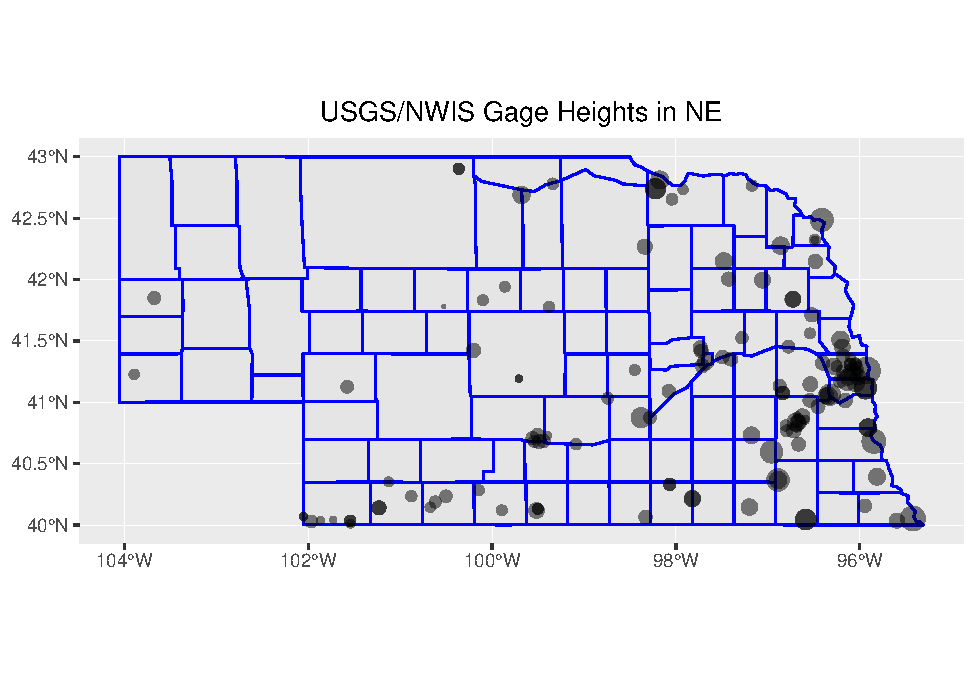
\includegraphics{A05_DataVisualization_files/figure-latex/unnamed-chunk-4-1.pdf}

\begin{enumerate}
\def\labelenumi{\arabic{enumi}.}
\setcounter{enumi}{5}
\tightlist
\item
  {[}USGS gauge{]} Plot discharge by date. Create two plots, one with
  the points connected with geom\_line and one with the points connected
  with geom\_smooth (hint: do not use method = ``lm''). Place these
  graphs on the same plot (hint: ggarrange or something similar)
\end{enumerate}

\begin{Shaded}
\begin{Highlighting}[]
\CommentTok{#6}

\CommentTok{# remove NAs in Stream.Raw}
\NormalTok{Stream.Raw_noNA <-}\StringTok{ }\NormalTok{Stream.Raw }\OperatorTok\StringTok{ }\KeywordTok{drop_na}\NormalTok{(X165986_00060_}\DecValTok{00001}\NormalTok{)}

\CommentTok{# find max value of max discharge (cubic feet per second)}
\KeywordTok{max}\NormalTok{(Stream.Raw_noNA}\OperatorTok{$}\NormalTok{X165986_00060_}\DecValTok{00001}\NormalTok{)}
\end{Highlighting}
\end{Shaded}

\begin{verbatim}
## [1] 4730
\end{verbatim}

\begin{Shaded}
\begin{Highlighting}[]
\CommentTok{# plot graph with geom_line}
\NormalTok{Discharge_bydate_line <-}\StringTok{ }\KeywordTok{ggplot}\NormalTok{(Stream.Raw_noNA, }\KeywordTok{aes}\NormalTok{(}\DataTypeTok{x =}\NormalTok{ datetime, }\DataTypeTok{y =}\NormalTok{ X165986_00060_}\DecValTok{00001}\NormalTok{)) }\OperatorTok{+}
\StringTok{  }\KeywordTok{geom_point}\NormalTok{() }\OperatorTok{+}
\StringTok{  }\KeywordTok{geom_line}\NormalTok{(}\DataTypeTok{color =} \StringTok{"blue"}\NormalTok{) }\OperatorTok{+}
\StringTok{  }\KeywordTok{xlab}\NormalTok{(}\OtherTok{NULL}\NormalTok{) }\OperatorTok{+}
\StringTok{  }\KeywordTok{ylab}\NormalTok{(}\KeywordTok{expression}\NormalTok{(}\KeywordTok{paste}\NormalTok{(}\StringTok{"Max Daily Discharge ("}\NormalTok{, ft}\OperatorTok{^}\DecValTok{3}\NormalTok{, }\StringTok{"/"}\NormalTok{, s,}\StringTok{")"}\NormalTok{, }\DataTypeTok{sep=}\StringTok{""}\NormalTok{))) }\OperatorTok{+}
\StringTok{  }\KeywordTok{ggtitle}\NormalTok{(}\StringTok{"USGS Streamflow data for site 02085000"}\NormalTok{)}
\KeywordTok{print}\NormalTok{(Discharge_bydate_line)}
\end{Highlighting}
\end{Shaded}

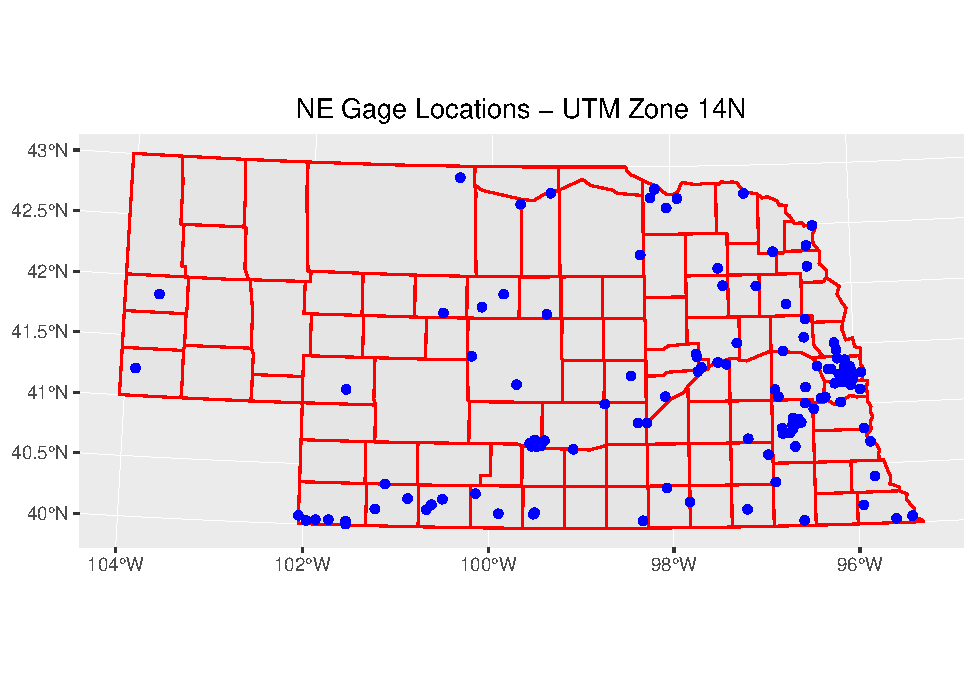
\includegraphics{A05_DataVisualization_files/figure-latex/unnamed-chunk-5-1.pdf}

\begin{Shaded}
\begin{Highlighting}[]
\CommentTok{# plot graph with geom_smooth}
\NormalTok{Discharge_bydate_smooth <-}\StringTok{ }\KeywordTok{ggplot}\NormalTok{(Stream.Raw_noNA, }\KeywordTok{aes}\NormalTok{(}\DataTypeTok{x =}\NormalTok{ datetime, }\DataTypeTok{y =}\NormalTok{ X165986_00060_}\DecValTok{00001}\NormalTok{)) }\OperatorTok{+}
\StringTok{  }\KeywordTok{geom_point}\NormalTok{() }\OperatorTok{+}
\StringTok{  }\KeywordTok{geom_smooth}\NormalTok{(}\DataTypeTok{method =} \StringTok{"auto"}\NormalTok{, }\DataTypeTok{color =} \StringTok{"orange"}\NormalTok{) }\OperatorTok{+}
\StringTok{  }\KeywordTok{ylab}\NormalTok{(}\KeywordTok{expression}\NormalTok{(}\KeywordTok{paste}\NormalTok{(}\StringTok{"Max Daily Discharge ("}\NormalTok{, ft}\OperatorTok{^}\DecValTok{3}\NormalTok{, }\StringTok{"/"}\NormalTok{, s,}\StringTok{")"}\NormalTok{, }\DataTypeTok{sep=}\StringTok{""}\NormalTok{)))}
\KeywordTok{print}\NormalTok{(Discharge_bydate_smooth)}
\end{Highlighting}
\end{Shaded}

\begin{verbatim}
## `geom_smooth()` using method = 'gam' and formula 'y ~ s(x, bs = "cs")'
\end{verbatim}

\includegraphics{A05_DataVisualization_files/figure-latex/unnamed-chunk-5-2.pdf}

\begin{Shaded}
\begin{Highlighting}[]
\CommentTok{# create combined figure}
\NormalTok{plot_stream <-}\StringTok{ }\KeywordTok{ggarrange}\NormalTok{(Discharge_bydate_line, Discharge_bydate_smooth,}
                         \DataTypeTok{ncol =} \DecValTok{1}\NormalTok{, }\DataTypeTok{nrow =} \DecValTok{2}\NormalTok{)}
\end{Highlighting}
\end{Shaded}

\begin{verbatim}
## `geom_smooth()` using method = 'gam' and formula 'y ~ s(x, bs = "cs")'
\end{verbatim}

\begin{Shaded}
\begin{Highlighting}[]
\KeywordTok{print}\NormalTok{(plot_stream)}
\end{Highlighting}
\end{Shaded}

\includegraphics{A05_DataVisualization_files/figure-latex/unnamed-chunk-5-3.pdf}
Question: How do these two types of lines affect your interpretation of
the data?

\begin{quote}
Answer: Interpreting the data with `geom\_line' makes the data appear to
be highly variable because this line type connects each data point with
the subsequent data point. Interpreting the data with geom\_smooth makes
the data seem relatively constant over time because this type creates a
line based on the frequency of data points at each value. For this
stream gauge, most of the data points were clustered around very low
data points, the trend line created is mostly constant, and sits at a
low daily discharge value.
\end{quote}

\begin{enumerate}
\def\labelenumi{\arabic{enumi}.}
\setcounter{enumi}{6}
\tightlist
\item
  {[}ECOTOX Neonicotinoids{]} Plot the concentration, divided by
  chemical name. Choose a geom that accurately portrays the distribution
  of data points.
\end{enumerate}

\begin{Shaded}
\begin{Highlighting}[]
\CommentTok{#7 }

\CommentTok{# filter to include only mg/L data}
\NormalTok{Neonicotinoids_mgL <-}\StringTok{ }
\StringTok{  }\NormalTok{Neonicotinoids.Raw }\OperatorTok
\StringTok{  }\KeywordTok{filter}\NormalTok{(Conc..Units..Std. }\OperatorTok{==}\StringTok{ "mg/L"}\NormalTok{)}

\NormalTok{Neonicotinoids_plot <-}
\StringTok{  }\KeywordTok{ggplot}\NormalTok{(Neonicotinoids_mgL, }\KeywordTok{aes}\NormalTok{(}\DataTypeTok{x =}\NormalTok{ Chemical.Name, }\DataTypeTok{y =}\NormalTok{ Conc..Mean..Std.)) }\OperatorTok{+}
\StringTok{  }\KeywordTok{geom_violin}\NormalTok{() }\OperatorTok{+}\StringTok{ }
\StringTok{  }\KeywordTok{xlab}\NormalTok{(}\StringTok{"Chemical Name"}\NormalTok{) }\OperatorTok{+}\StringTok{ }
\StringTok{  }\KeywordTok{ylab}\NormalTok{(}\StringTok{"Concentration (mg/L)"}\NormalTok{) }\OperatorTok{+}\StringTok{ }
\StringTok{  }\KeywordTok{ggtitle}\NormalTok{(}\StringTok{"Concentration (mg/L) of 5 Neonicotinoids"}\NormalTok{)}
\KeywordTok{print}\NormalTok{(Neonicotinoids_plot)}
\end{Highlighting}
\end{Shaded}

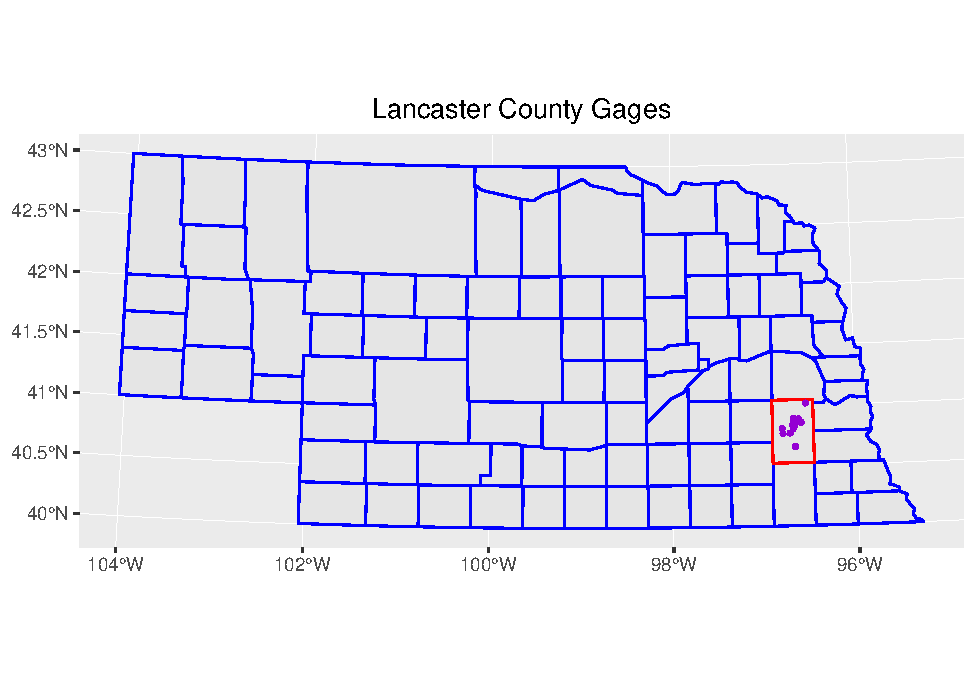
\includegraphics{A05_DataVisualization_files/figure-latex/unnamed-chunk-6-1.pdf}


\end{document}
